\documentclass[11pt,a5paper]{article}
\usepackage{amsmath,parskip,enumitem,pgfplots}
\pgfplotsset{compat=newest}
%\usepgfplotslibrary{patchplots}% for "patch refines"
%\usepackage{pgfplotstable} % for some table plots
% view stereo with cross eyes, or vice-versa
%\newcommand{\qview}[2]{\foreach \q in {#2,#1}}
\newcommand{\answer}[1]{} % do nothing with answers
\renewcommand{\vec}[1]{\text{\boldmath$#1$}}
\renewcommand{\Vec}[1]{%
  \expandafter\def\csname#1v\endcsname%
  {\ensuremath{\vec #1}}}


\title{Exercise \jobname}
\author{A. J. Roberts, \today}
\date{}

\begin{document}

\maketitle

\def\svd{\textsc{svd}}
The picture shows a \(7\times5\) pixel image of the letter~\texttt{G}.
Compute an \svd\ of the pixel image.
By inspecting various rank approximations from this \svd, determine the rank of the approximation to~\texttt{G} shown.

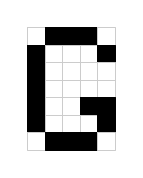
\begin{tikzpicture}
\begin{axis}[tiny,axis equal image
,colormap/blackwhite,axis lines=none]
\addplot[patch,patch type=rectangle
,point meta min={0},point meta max={ 1.000}
,table/row sep=\\,patch table with point meta={
0 1 9 8  1.000 \\
1 2 10 9  0.000 \\
2 3 11 10  0.000 \\
3 4 12 11  0.000 \\
4 5 13 12  0.000 \\
5 6 14 13  0.000 \\
6 7 15 14  1.000 \\
8 9 17 16  0.000 \\
9 10 18 17  1.000 \\
10 11 19 18  1.000 \\
11 12 20 19  1.000 \\
12 13 21 20  1.000 \\
13 14 22 21  1.000 \\
14 15 23 22  0.000 \\
16 17 25 24  0.000 \\
17 18 26 25  1.000 \\
18 19 27 26  1.000 \\
19 20 28 27  1.000 \\
20 21 29 28  1.000 \\
21 22 30 29  1.000 \\
22 23 31 30  0.000 \\
24 25 33 32  0.000 \\
25 26 34 33  1.000 \\
26 27 35 34  1.000 \\
27 28 36 35  1.000 \\
28 29 37 36  0.000 \\
29 30 38 37  1.000 \\
30 31 39 38  0.000 \\
32 33 41 40  1.000 \\
33 34 42 41  0.000 \\
34 35 43 42  1.000 \\
35 36 44 43  1.000 \\
36 37 45 44  0.000 \\
37 38 46 45  0.000 \\
38 39 47 46  1.000 \\
}]
table[row sep=\\] {
x y \\
0 7 \\
0 6 \\
0 5 \\
0 4 \\
0 3 \\
0 2 \\
0 1 \\
0 0 \\
1 7 \\
1 6 \\
1 5 \\
1 4 \\
1 3 \\
1 2 \\
1 1 \\
1 0 \\
2 7 \\
2 6 \\
2 5 \\
2 4 \\
2 3 \\
2 2 \\
2 1 \\
2 0 \\
3 7 \\
3 6 \\
3 5 \\
3 4 \\
3 3 \\
3 2 \\
3 1 \\
3 0 \\
4 7 \\
4 6 \\
4 5 \\
4 4 \\
4 3 \\
4 2 \\
4 1 \\
4 0 \\
5 7 \\
5 6 \\
5 5 \\
5 4 \\
5 3 \\
5 2 \\
5 1 \\
5 0 \\
};
\end{axis}
\end{tikzpicture}





\end{document}
